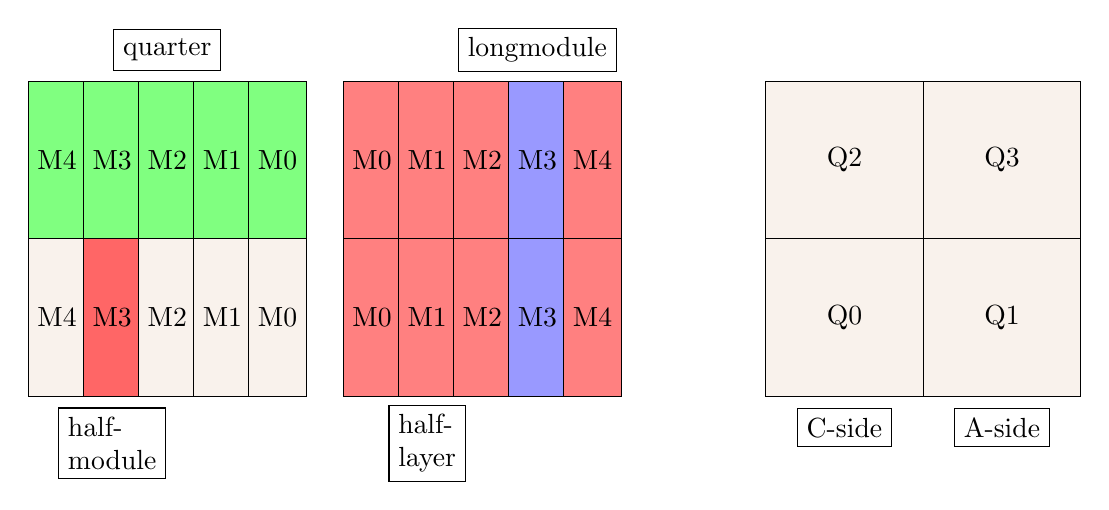
\begin{tikzpicture}
% first quarter
  \node[rectangle,
      draw = black,
      % text = ,
      fill = brown!10!white,
      minimum width = 0.7cm,
      minimum height = 2cm] (r) at (0,0) {M4};

  \node[rectangle,
      draw = black,
      % text = half-module,
      fill = red!60!white,
      minimum width = 0.7cm,
      minimum height = 2cm] (r) at (0.7,0) {M3};

  \node[rectangle,
      draw = black,
      % text = ,
      fill = brown!10!white,
      minimum width = 0.7cm,
      minimum height = 2cm] (r) at (1.4,0) {M2};

  \node[rectangle,
      draw = black,
      % text = ,
      fill = brown!10!white,
      minimum width = 0.7cm,
      minimum height = 2cm] (r) at (2.1,0) {M1};

  \node[rectangle,
      draw = black,
      % text = ,
      fill = brown!10!white,
      minimum width = 0.7cm,
      minimum height = 2cm] (r) at (2.8,0) {M0};

% second quarter
\node[rectangle,
    draw = black,
    % text = ,
    fill = red!50!white,
    minimum width = 0.7cm,
    minimum height = 2cm] (r) at (4,0) {M0};

\node[rectangle,
    draw = black,
    % text = ,
    fill = red!50!white,
    minimum width = 0.7cm,
    minimum height = 2cm] (r) at (4.7,0) {M1};

\node[rectangle,
    draw = black,
    % text = ,
    fill = red!50!white,
    minimum width = 0.7cm,
    minimum height = 2cm] (r) at (5.4,0) {M2};

\node[rectangle,
    draw = black,
    % text = ,
    fill = blue!40!white,
    minimum width = 0.7cm,
    minimum height = 2cm] (r) at (6.1,0) {M3};

\node[rectangle,
    draw = black,
    % text = ,
    fill = red!50!white,
    minimum width = 0.7cm,
    minimum height = 2cm] (r) at (6.8,0) {M4};

% third quarter
\node[rectangle,
    draw = black,
    % text = ,
    fill = green!50!white,
    minimum width = 0.7cm,
    minimum height = 2cm] (r) at (0,2) {M4};

\node[rectangle,
    draw = black,
    % text = quarter,
    fill = green!50!white,
    minimum width = 0.7cm,
    minimum height = 2cm] (r) at (0.7,2) {M3};

\node[rectangle,
    draw = black,
    % text = ,
    fill = green!50!white,
    minimum width = 0.7cm,
    minimum height = 2cm] (r) at (1.4,2) {M2};

\node[rectangle,
    draw = black,
    % text = ,
    fill = green!50!white,
    minimum width = 0.7cm,
    minimum height = 2cm] (r) at (2.1,2) {M1};

\node[rectangle,
    draw = black,
    % text = ,
    fill = green!50!white,
    minimum width = 0.7cm,
    minimum height = 2cm] (r) at (2.8,2) {M0};

% fourth quarter
\node[rectangle,
    draw = black,
    % text = ,
    fill = red!50!white,
    minimum width = 0.7cm,
    minimum height = 2cm] (r) at (4,2) {M0};

\node[rectangle,
    draw = black,
    % text = ,
    fill = red!50!white,
    minimum width = 0.7cm,
    minimum height = 2cm] (r) at (4.7,2) {M1};

\node[rectangle,
    draw = black,
    % text = ,
    fill = red!50!white,
    minimum width = 0.7cm,
    minimum height = 2cm] (r) at (5.4,2) {M2};

\node[rectangle,
    draw = black,
    % text = ,
    fill = blue!40!white,
    minimum width = 0.7cm,
    minimum height = 2cm] (r) at (6.1,2) {M3};

\node[rectangle,
    draw = black,
    % text = ,
    fill = red!50!white,
    minimum width = 0.7cm,
    minimum height = 2cm] (r) at (6.8,2) {M4};

\node[draw, align=left] at (1.4, 3.4) {quarter};
\node[draw, align=left] at (0.7, -1.6) {half-\\module};
\node[draw, align=left] at (4.7, -1.6) {half-\\layer};
\node[draw, align=left] at (6.1, 3.4) {longmodule};

% label quarters
\node[rectangle,
    draw = black,
    % text = Q2,
    fill = brown!10!white,
    minimum width = 2cm,
    minimum height = 2cm] (r) at (10,0) {Q0};

\node[rectangle,
    draw = black,
    % text = Q3,
    fill = brown!10!white,
    minimum width = 2cm,
    minimum height = 2cm] (r) at (12,0) {Q1};

\node[rectangle,
    draw = black,
    % text = Q0,
    fill = brown!10!white,
    minimum width = 2cm,
    minimum height = 2cm] (r) at (10,2) {Q2};

\node[rectangle,
    draw = black,
    % text = Q1,
    fill = brown!10!white,
    minimum width = 2cm,
    minimum height = 2cm] (r) at (12,2) {Q3};

\node[draw, align=left] at (10, -1.4) {C-side};
\node[draw, align=left] at (12, -1.4) {A-side};

\end{tikzpicture}
